\section{Neural Networks}

A Neural Network is an information processing paradigm that is inspired by the way biological nervous systems, such as the brain, process information. The key element of this paradigm is the new structure of the information processing system. It is composed of a large number of highly interconnected processing elements (\textbf{neurons}) working in unison to solve specific problems. A NN is configured for a specific application, such as pattern recognition or data classification, through a learning process.\\
Two key \textbf{features} distinguish neural networks from any other sort of computing developed:

\begin{itemize}
	\item \textbf{Neural networks are adaptive or trainable}. Neural networks are not so much programmed as they are trained with data. The more data they are fed, the more accurate or complete is their response;
	\item \textbf{Neural network are naturally massively parallel}. This suggests they should be able to make decisions at high-speed and be fault tolerant (information is stored in a distributed fashion). 
\end{itemize}

\subsection{Biological digression}
As we introduced before, the functioning of a Neural Network is highly inspired by the way in which the neural system and the brain process the information. The biological neural network is composed by the following elements:

\image{img/neural_dynamics}{Neural dynamics.}{0.6}


\begin{itemize}
	\item \textbf{Cell body (Soma)}: 5-10 microns in diameter, it represents the \textit{computational unit};
	\item \textbf{Axon}: it represents the output mechanism for a neuron. A single axon may be connected to thousands of branches and cells;
	\item \textbf{Dendrites}: they receive incoming signals from other nerve axons via synapse;
	\item \textbf{Synapses}: they represents the junctions (``connecting points'') between neurons, i.e. the point in which a neuron's axon passes the information to the "next" neuron's dendrite.
\end{itemize}

The \textbf{transmission of signal} in the cerebral cortex is a complex process:
$$\text{Electrical} \rightarrow \text{Chemical} \rightarrow \text{Electrical}$$
Simplifying:
\begin{enumerate}
	\item The cellular body performs a "\textit{weighted sum}" of the incoming signals.
	\item If the result exceeds a certain threshold value, then it produces an "action potential" which is sent down the axon (cell has "fired"), otherwise it remains in a rest state.
	\item When the electrical signal reaches the synapse, it allows the ``neuro-transmitter'' (chemical) to be released. This combines with the ``receptors'' in the post-synaptic membrane.
	\item The post-synaptic receptors provoke the diffusion of an electrical signal in the post-synaptic neuron. 
\end{enumerate}
In summary, computations by neuron are performed thanks to a combination of electrical and chemical processes. 

A very important concept of the neural system is the so-called \textbf{synaptic efficacy}, which can be defined as the amount of electricity that enters into the post-synaptic neuron, compared to the action potential of the pre-synaptic neuron. The \textbf{learning step} takes place by modifying the synaptic efficacy. In general, two different types of synapses are present:
\begin{itemize}
	\item \textbf{Excitatory}, which favor the generation of action potential in the post-synaptic neuron, i.e. they tend to increase the energy;
	\item \textbf{Inhibitory}, which hinder the generation of action potential, so they de-amplify the signal.
\end{itemize}

\subsection{The McCulloch and Pitts Model (1943)}

Neural network simulations appear to be a recent development; however, this field was established before the advent of computers and the first model, which was created in 1943, is the \textbf{McCulloch and Pitts Model}.\\
The McCulloch-Pitts (MP) neuron is a simple process unit modeled as a binary threshold unit.

\image{img/MP_neuron}{McCulloch and Pitts neuron representation.}{0.55}


\textbf{Input} = $x$ = $\sum_j w_jI_j$. \\
\textbf{Output} = $g(x) = \begin{cases}
0 \quad \text{if }x<T\\
1 \quad \text{if }x \geq T
\end{cases}$

In this sense, we can rewrite the output as:

$$
y = g\left(\sum_j w_jI_j - T\right) 
$$

\textbf{NOTE}:

\begin{itemize}
    \item the MP neuron fires if the input $x$ = $\sum_j w_jI_j$ exceeds a certain threshold $T$, called \textbf{claiming parameter};

    \item the function $g(.)$ is also called \textbf{activation function} or \textbf{unit step function}, and it is a non linear function;

    \item the weight $w_{ij}$ represents the strength of the synapse between neuron $i$ and neuron $j$. 
\end{itemize}

\subsubsection{Properties}

By properly combining MP neurons, it is possible to simulate the behavior of any boolean circuit:

\image{img/MP_properties}{Three elementary logical operations (\textit{a}) \textbf{negation}, (\textit{b}) \textbf{and}, (\textit{c}) \textbf{or}. In each diagram the states of the neurons on the left are at time $t$ and those on the right at time $t+1$.}{0.65}

Notice that it is not possible to build a NN for the \textit{XOR} operator using a single neuron.

\subsection{Network topologies and Architectures} There are different network topologies and the main differences are highlighted below.

\begin{table}[H]
	\centering
	\begin{tabular}{| p{7.5cm} | p{7.5cm} |}
		\hline
		\textbf{Feed-forward only}: allow signals to travel one way only: from input to output, so it has connections only in one direction. This topology forms a direct acyclic graph, and its outputs are deterministic functions of the input & \textbf{Recurrent networks}: can have signals traveling in both directions by introducing loops in the network. Feedback networks are powerful and can get extremely complicated, since their output depends on the initial state, which in turn depends on previous outputs.\\
		\hline
		\textbf{Fully connected}: each neuron of a layer is connected to every neuron in the previous layer, and each connection has it's own weight. & \textbf{Sparsely connected}: has fewer links than the possible maximum number of links within that network.  \\
		\hline
		\textbf{Single layer}: every neuron connects directly from the network's input to its output & \textbf{Multi-layer}: it has one or more layer of hidden neurons that are not connected to the output.\\
		\hline
	\end{tabular}
\end{table} 
\image{img/feedforward}{\textit{(a)} feedforward network - \textit{(b)} feedback network}{0.65}

In general, there are problems which are more suited to be solved with a \textit{feedforward NN} than a \textit{recurrent NN} or vice-versa, for example a task of image classification, i.e. assigning a label to an input image, can be easily solved with a \textit{feedforward NN}, whereas a task of image captioning, i.e. provide a verbal description of the input image, is more suitable to be solved with a \textit{recurrent NN}, since the length of the output is not known in advance. 


\subsection{Classification problems}
Given:

\begin{enumerate}

	\item a set of \textbf{features} $\{f_1,f_2,\dots,f_n\}$ , which represents the attributes that describe our objects;
	\item a set of \textbf{classes} $\{c_1,\dots,c_m\}$, which represents the categories in which the objects are divided
 
\end{enumerate}

, the \textbf{goal} of the \textbf{classification} problem is to classify the \textbf{objects} according to their \textbf{features}. The geometric interpretation of this task is to represent the features in the space and try to separate the classes by finding the closest objects.

\image{img/nn1.jpg}{Classification problem}{0.7}

\subsubsection{Neural networks for classification}

A neural networks can be used as a classification device and it can be configured as follow:

\begin{itemize}

	\item the \textit{input} of the network are the object's \textbf{features} to classify.
 
	\item the \textit{output}, returned by the network, is the \textbf{class} predicted for the input object.
 
\end{itemize}

Before going on we assume that features are numbers, and remember that we cannot map categorical features into numbers, since we would introduce an order, which would lead to mistakes. For instance: red = 0, blue = 1, green = 2 would not be a correct coding since we would be imposing a non-existent order between colors. We propose a simple model of neural network:

\image{img/NN_1}{Example of NN with 3 features input and 2 class labels as output.}{0.4}

The application of a learning algorithm of a network configuration consists in finding the best configuration of weights of the incoming connection and the threshold. In these classification problems we can get rid of the \textbf{thresholds} (also called biases) associated to neurons by adding an extra input \textbf{permanently clamped at -1}. By doing so,\textbf{ thresholds become weights} and can be adaptively adjusted during learning phase, otherwise we would have to manually tune the right threshold. In this way, the output $y$ of the network becomes:

$$
y = g\left(\sum\limits_{i = 1}^{n+1} w_ix_i\right)
$$
, where $x_{n+1} = -1$.

\begin{figure}[h!]
		\centering
        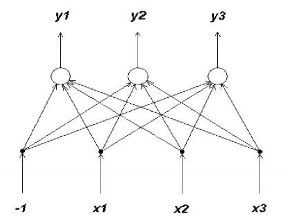
\includegraphics[scale = 1.5]{img/thresholds.jpg}
		\label{mi}
        \caption{We can remove thresholds by adding an input neuron clamped at -1}
\end{figure}

\subsubsection{The Perceptron}
The perceptron is a \textbf{linear classifier} consisting of a \textbf{single layer of MP neurons} connected in a \textbf{feedforward} way, i.e. it is a \textbf{single-layer feedforward NN}. A simple perceptron can only solve linearly separable problems, and this makes the model very limited in terms of computational power. 

\image{img/percep1.jpg}{Representation of a perceptron}{0.5}

The perceptron is characterized by the following properties:

\begin{itemize}
    \item The output is $-1/+1$, while using the MP neurons we had $0/1$;
    
    \item It is capable of learning from examples;
    
    \item From a geometrical point of view, the perceptron identifies a linear boundary between two classes:

    \image{img/percep2.jpg}{Geometry interpretation of the perceptron}{0.5}

    In this case, the hyperplane (line) $w_1x_1 + w_2x_2 - b$ represents a linear decision boundary for a two-dimensional, two-classes classification problem. If $w_1x_1 + w_2x_2 - b > 0$ then the predicted class is 1, otherwise is 0. Obviously, if we change the parameters $w_1$, $w_2$ and $b$, we get a different boundary.
    
\end{itemize}

\paragraph*{The Perceptron Learning Algorithm.} The goal of this algorithm is to find the best weights and parameters in order to separate the objects of the classes. It is an iterative algorithm characterized by the following variables and parameters:
\begin{itemize}

	\item $x(n) \in \mathbb{R}^{m+1}$, the \textbf{input vectors}. They are $(m+1)\text{-by-1 vectors} = [-1, x_1(n), x_2(n), \dots, x_m(n)]^T$\\
	Objects are described with $m$ features and -1 as the threshold, which is the reason why the input vectors have size $m+1$;
 
	\item $w(n) \in \mathbb{R}^{m+1}$, the \textbf{weights vectors}. They are $(m+1)\text{-by-1 vectors} = [b, w_1(n), w_2(n), \dots, w_m(n)]^T$;
 
	\item $b$, the \textbf{bias};
 
	\item $y(n)$, the \textbf{actual response} of the NN (quantized). $y(n) \in \{ +1, -1 \}$;
 
	\item $d(n)$, the \textbf{desired response} from the dataset. $d(n) \in \{ +1, -1 \}$;
 
	\item $\eta$, the \textbf{learning-rate parameter}, a positive constant strictly smaller than $1$. It affects the convergence of the learning algorithm. 
\end{itemize}

The algorithm works as follows:

\begin{enumerate}

	\item \textbf{Initialization.} Set $w(0) = 0$ and then perform the following computations for time-step $n=1,2,\dots$.
 
	\item \textbf{Activation.} At time-step $n$, activate the perceptron by applying continuous-valued input vector $x(n)$ and desired response $d(n)$ (both picked from the training set).
 
	\item \textbf{Computation of the actual response.} Compute the actual response of the perceptron as:
	$$y(n) = sgn[w^T(n)x(n)] \qquad w^Tx = \sum_iw_ix_i$$
	where $sgn(\cdot)$ is the signum function ($+1$ if the argument is greater or equal to $0$, $0$ otherwise). Notice that, so far, no learning phase has taken place.
 
	\item \textbf{Update of the weight vector.} Update the weight vector of the perceptron to obtain:
	$$w(n+1) = w(n) + \eta[d(n) - y(n)]x(n)$$
	where
	$$d(n) = 
	\begin{cases}
	+1 \qquad \text{if } x(n) \text{ belongs to class } \varphi_1\\
	-1 \qquad \text{if } x(n) \text{ belongs to class } \varphi_2 
	\end{cases}$$
	This is where the learning phase takes place: in case of wrong classification, the current configuration will change modifying $d(n) - y(n)$, if the network classifies $x(n)$ correctly, then there is no learning as $d(n)-y(n) = 0$. The convergence of the algorithm is ensured by $x(n)$. Note that $x(n)$ is included to be sure that the new prediction is correct, but the updated weights could fail to classify another input vector (even an already seen one).
 
	\item \textbf{Continuation.} Increment time step $n$ by one and go back to step 2.
 
\end{enumerate}

In practice, this algorithm is trying to find the best possible straight line (or hyperplane) which separates the ``good'' examples from the ``bad'' ones. The decision boundary is described such that $w_1x_1 + w_2x_2 = 0$ and, in general, each point is classified according to the following conditions:  $w_1x_1 + w_2x_2 \geq 0$ and $w_1x_1 + w_2x_2 < 0$

\image{img/perceptron_algorithm}{Perceptron learning algorithm procedure.}{0.50}

From a geometrical point of view, finding $w$ means finding the line (or hyperplane) which separates the two regions.
As we can see from the previous image, some examples can be misclassified. For each weights update, a specific error is corrected but other mistakes in classification may arise because of the changes in the weights. By iteratively adjusting the weights, a final and ``stable'' solution can be reached.\\
It is possible to define a \textbf{decision region} as an area in which all the samples of one class fall. A classification problem is said to be \textbf{linearly separable} if the decision regions can be separated by an hyperplane. These concepts allow us to introduce one important \textbf{limitation of perceptrons}: they can only solve linearly separable problems.

\paragraph*{The Perceptron Convergence Theorem.} This theorem was formulated by Rosenblatt in 1960. It states the following: if the training set is \textbf{linearly separable}, the perceptron learning algorithm \textbf{always converges} to a consistent hypothesis after a \textbf{finite} number of epochs, i.e. an entire presentation of the dataset, for any $\eta > 0$ (Note: nothing is said with respect to the number of steps).\\
If the training set is \textbf{not linearly separable}, after a certain number of epochs the weights will start oscillating. In this situation some points will surely be misclassified. The learning algorithm will never converge to a stable configuration, due to the fact that the perceptron can't solve non-linear classification problems.

\par \bigskip \noindent
\subsection{Multi-Layer Feed-forward Neural Networks}
In the following image it is possible to find some properties of the different structures that can create a neural network.

\image{img/role_units}{A view of the Role of Units}{0.86}

As we said before, the limit of the perceptron algorithm is that it can only deal with linearly separable problems. In order to overcome these limitations, the introduction of \textbf{multi-layer feed-forward networks} allows us to improve our networks through the addition of \textbf{hidden layers} between the input and the output layer. This allows us to reach a good approximation on our classification problem: it is possible to notice that a network with just one hidden layer can represent any Boolean function, including XOR. One property of such networks is the \textbf{universal approximation power}, which states that a 2-layers network (one input layer, one hidden layer) can approximate any smooth function (valid for regression problems), provided that the hidden layer is large enough.

\image{img/fNN.png}{Neural Network function model.}{0.65}		


\paragraph*{Continuous-valued units.} The usage of continuous-valued units allows us to introduce calculus and derivative procedures that will give us several advantages.\\ 
The \textbf{activation function} of continuous-valued units is \textbf{sigmoid} (or logistic), which means that neurons can now fire with different intensities, not only 0/1. In this sense, their output is not boolean, but it belongs to the continuous range between $0$ and $1$. These values are often interpreted as probabilities.
$$g \rightarrow \sigma(x) = \frac{1}{1+e^{-f(x)}} \in (0,1)$$
\image{img/sigmoid}{Sigmoid function.}{0.51}
Thus, continuous-valued discriminant functions allow us to have some measure of \textbf{confidence} about the \textbf{prediction}. We will see later on that they are used for \textbf{finding optimal solutions through the gradient descent technique}. In particular, when the $g(z)$ is close to zero (less confidence about the prediction) the gradient will be greater then the situation in which $|g(x)| >> 0$ (more confidence, weights could remain stable).

Another possible activation function is the \textbf{hyperbolic tangent} ($tanh$), which is a rescaling of the logistic sigmoid such that its output range is from -1 and 1. 
$$g \rightarrow \sigma(x) = \frac{e^{f(x)} - e^{-f(x)}}{e^{f(x)} + e^ {-f(x)}} \in (-1, 1)$$
\image{img/hyperbolic}{Hyperbolic tangent function.}{0.45}


\subsection{Back-propagation learning algorithm}
In this section we introduce the \textbf{backpropagation}, an algorithm for learning the weights in a feed-forward multilayers neural network. 

Let $\mathcal{L} = \{(x_1, y_1), \dots, (x_n,y_n) \}$ be a \textbf{training set}, where $X = \{ x_1, x_2, .., x_n \}$ represents the network \textbf{input} vector and $Y = \{ y_1, y_2, .., y_n \}$ represents the \textbf{desired} network \textbf{output} vector. The algorithm is based on \textbf{gradient descent} method, and it can be seen as a greedy algorithm with infinite possible solutions, in which at each step the best solution is chosen. The algorithm is guaranteed to converge only to a local maximum and during the execution we move along the gradient through a predetermined step-size. This property is given by the fact that this algorithm is just an approximation based on a greedy solution.

\image{img/backpropagation}{Back-propagation schema. $W^l_{ij}$ represents the weight on connection between the $i^{th}$ unit in layer $(l-1)$ to $j^{th}$ unit in layer $l$.}{0.70}

\paragraph*{Supervised learning.} Supervised learning algorithms require the presence of \textbf{previous knowledge} that makes it possible to provide the \textbf{right answers} to the input ``questions''. Technically this means that we need a \textbf{training set} of the form:

$$
\mathcal{L} =\left\{\left(x^1, y^1 \right), \dots , \left(x^N, y ^N \right) \right\}
$$

where:

$$x^\mu (\mu=1,\dots, N) \text{ is the network \textbf{input} vector}$$
$$y^\mu (\mu=1,\dots, N) \text{ is the \textbf{desired} network \textbf{output} vector}$$

The learning (or \textbf{training}) phase consists in determining a configuration of \textbf{weights} such that the \textbf{network output} should be \textbf{as close as possible} to the \textbf{desired output} as many times as possible, for all the examples in the training set. Normally, this amounts to minimizing an \textbf{error function} such as the \textbf{MSE} (Mean Squared Error) function:
$$E(w) = \frac{1}{2} \sum_{\mu} \sum_{k} \left(y_k^\mu - O_k^\mu(w)\right)^2$$
where $O_k^\mu(w)$ is the \textbf{output} provided by the \textbf{output unit $k$} when the network is given example $\mu$ as \textbf{input}. In other words, $O_k^\mu(w)$ represents the prediction of the $k^{th}$ unit when the input is $\mu$. 

The loss function computes the difference between the network output and the expected output and of course, our aim is to \textbf{minimize the loss function} (i.e. solve $min_w E(w)$), which means \textbf{finding the set of weights that minimizes the function}: if the network is performing well, then $E(w$ is close to zero.

In order to minimize the error function $E$, we can use the classic \textbf{gradient descent} algorithm. The gradient gives information about the \textbf{best path to follow} in order to \textbf{maximize/minimize our objective function}. Without any kind of direction information it would be extremely complex to find the solution since we would have to search along an infinite number of directions in a continuous domain. Gradient descent is a very well-known \textbf{greedy algorithm}. It is not guaranteed to find a globally optimal solution, but it works well in finding \textbf{local optima}. 

More specifically, the gradient descent updates the a point by moving along the the direction given by the gradient by a finite step. In the case of the back-propagation algorithm, we have that:
$$w_{ji}^{\text{NEW}} \leftarrow w_{ji}^{\text{OLD}} - \eta \frac{\partial E}{\partial w_{ji}}$$

or

$$\Delta w_{ji} \leftarrow  - \eta \frac{\partial E}{\partial w_{ji}^{\text{OLD}}}$$

, where :

\begin{itemize}
    \item $\Delta w_{ji} = w_{ij}^{\text{NEW}} - w_{ji}^{\text{OLD}}$
    \item $w_{ji}^{\text{NEW}}$ represent the weights between unit $i$ and unit $j$, and they are updated using the gradient of the loss function $E$ computed w.r.t. $w_{ji}^{\text{OLD}}$;
    \item $\eta$ represents the \textbf{learning rate}, i.e. how much the weights are updated at each iteration of the gradient descent method. We will discuss about the possible values of this parameter later in the section;
\end{itemize}

Now we need to define a method for computing the partial derivatives of the loss function efficiently.

To compute the partial derivatives we use the \textbf{error back propagation} algorithm, which consists of two stages:

\begin{itemize}
	\item \textbf{Forward pass}: the \textbf{input} of the network is \textbf{propagated} layer after layer in \textbf{forward} direction.
	\item \textbf{Backward pass}: the \textbf{error} (e.g. MSE) made by the network is \textbf{propagated} \textbf{backward} and \textbf{weights} are \textbf{updated} properly. Thus, the partial derivatives of the errors are computed, and the weights are updated following the gradient descent strategy we defined above. An important thing to underline is that in order to update each weight, we only need a \textbf{local information}, not a global information of all the network.
\end{itemize}


Intuitively, we could say that we determine the gradient direction and then we move in the opposite direction since we want to minimize the error.

\paragraph*{Notation.} Before understanding how the weights are updated, it is important to introduce some notation that will be used later:

\begin{itemize}
    \item $x_k$ represents an input neuron of the network;
    \item $w_{jk}$ represents a weight between the input $x_k$ and the neuron $V_j$ in the middle layer;
    \item $V_j$ represents a neuron in the hidden layer;
    \item $W_{ij}$ represents a weight between a neuron in the hidden layer $V_j$ and the output neuron $O_i$;
    \item $O_i$ represents a output neuron.
\end{itemize}

\imageb{img/notations}{0.5}

Given a pattern $\mu$, an hidden unit $j$ receives a net input
$$h _ { j } ^ { \mu } = \sum _ { k } w _ { j k } x _ { k } ^ { \mu }$$
and produces as output:
$$V _ { j } ^ { \mu } = g \left( h _ { j } ^ { \mu } \right) = g \left( \sum _ { k } w _ { j k } x _ { k } ^ { \mu } \right)$$
The output of a neuron in the output layer is defined as:
$$O _ {i} ^ {\mu} = g(\sum _ k W_{ik} \cdot V _ {k} ^ {\mu})$$


\paragraph*{Updating hidden-to-output weights.} The \textbf{updating rules} of the back-propagation algorithm are nothing but a \textbf{long series of chain rules}. For this reason, the objective function is not linear, hence the output is highly non linear. Indeed, the output is a chain of products of non-linear functions.\\
\begin{equation} \notag
\begin{split}
\Delta W_{ij} &= -\eta \frac{\partial E}{\partial W_{ij}} \quad \text{Replace the error function with its actual expression}\\
&= -\eta \frac{\partial}{\partial W_{ij}} \left[\frac{1}{2} \sum_{\mu} \sum_k (y_k^\mu - O_k^\mu)^2\right] \quad \text{First application of the chain rule}\\
&= \eta \sum _{\mu} \sum_{k} \left(y_{k}^{\mu} - O_{k}^{\mu} \right) \frac{\partial O_{k}^{\mu}} {\partial W_{ij}} \quad \text{The sum over } k \text{ disappears because the partial derivative is}\\
& \hspace*{13.5em} \text{different from 0 only when }k=i \\
&= \eta \sum_{\mu} \left(y_{i}^{\mu} - O_{i}^{\mu} \right) \frac{\partial O_{i}^{\mu}} {\partial W_{ij}} \qquad \text{Again we apply the chain rule. Partial derivative can be}\\
& \hspace*{12.6em} \text{written as } W_{ij} \rightarrow h_i^\mu \rightarrow g'(h_i^\mu)\\
&= \eta \sum _ { \mu } \left( y _ { i } ^ { \mu } - O _ { i } ^ { \mu } \right) g ^ { \prime } \left( h _ { i } ^ { \mu } \right) V _ { j } ^ { \mu } \qquad \text{That is } \frac{\partial h_i^\mu}{\partial W_{ij}} = \frac{\partial}{\partial W_{ij}}\left(\sum_l W_{il} V_l \right) = V_j \frac{\partial W_{ij}}{\partial W_{ij}} = V_j\\
&= \eta \sum _ { \mu } \delta _ { i } ^ { \mu } V _ { j } ^ { \mu } \qquad \qquad where: \quad \delta _ { i } ^ { \mu } = \left( y _ { i } ^ { \mu } - O _ { i } ^ { \mu } \right) g ^ { \prime } \left( h _ { i } ^ { \mu } \right)
\end{split}	
\end{equation}
In $\eta \sum_{\mu} \delta_{i}^{\mu} V_{j}^{\mu}$, component $\delta_{i}^{\mu}$ represents the error made by the $i$-th neuron, whilst $V_{j}^{\mu}$ is the output of the neuron.  

\paragraph*{Updating input-to-hidden weights.}
\begin{equation} \notag
\begin{split}
\Delta w _ { j k } &= - \eta \frac { \partial E } { \partial w _ { j k } } \\
&= \eta \sum _ { \mu } \sum _ { i } \left( y _ { i } ^ { \mu } - O _ { i } ^ { \mu } \right) \frac { \partial O _ { i } ^ { \mu } } { \partial w _ { j k } } \qquad \text{Chain rule}\\
&= \eta \sum _ { \mu } \sum _ { i } \left( y _ { i } ^ { \mu } - O _ { i } ^ { \mu } \right) g ^ { \prime } \left( h _ { i } ^ { \mu } \right) \frac { \partial h _ { i } ^ { \mu } } { \partial w _ { j k } } \qquad \text{Chain rule}
\end{split}
\end{equation}
We have that the partial derivative is:
\begin{equation} \notag
\begin{split}
\frac { \partial h _ { i } ^ { \mu } } { \partial w _ { j k } } &= \sum _ { l } w_{ i l } \frac { \partial V _ { l } ^ { \mu } } { \partial w_{ j k } }\\
&= w_ { i j } \frac { \partial  V_ { j } ^ { \mu } } { \partial  w _ { j k } }\\
&= w_{ i j } \frac { \partial g \left( h _ { j } ^ { \mu } \right) } { \partial w _ { j k } }\\
&= w_{ i j } g ^ { \prime } \left( h _ { j } ^ { \mu } \right) \frac { \partial h _ { j } ^ { \mu } } { \partial w _ { j k } }\\
&= w_{ i j } g ^ { \prime } \left( h _ { j } ^ { \mu } \right) \frac { \partial } { \partial w _ { j k } } \sum _ { m } w _ { j m } x _ { m } ^ { \mu }\\
&=  w_{ i j } g ^ { \prime } \left( h _ { j } ^ { \mu } \right) x _ { k } ^ { \mu }
\end{split}
\end{equation}
Hence coming back to the original equation we have that:
\begin{equation}
\begin{split}
\Delta w _ { j k } &= \eta \sum _ { \mu , i } \left( y _ { i } ^ { \mu } - O _ { i } ^ { \mu } \right) g ^ { \prime } \left( h _ { i } ^ { \mu } \right) w_ { i j } ~g ^ { \prime } \left( h _ { j } ^ { \mu } \right) x _ { k } ^ { \mu }\\
&= \eta \sum _ { \mu , i } \delta _ { i } ^ { \mu } w_ { i j } g ^ { \prime } \left( h _ { j } ^ { \mu } \right) x _ { k } ^ { \mu }\\
&= \eta \sum _ { \mu } \hat { \delta } _ { j } ^ { \mu } x _ { k } ^ { \mu } \qquad \qquad where: \quad \hat { \delta } _ { j } ^ { \mu } = g ^ { \prime } \left( h _ { j } ^ { \mu } \right) \sum _ { i } \delta _ { i } ^ { \mu } w_ { i j }
\end{split}
\end{equation}
$\sum_{i} \delta_{i}^{\mu} W_{ij}$ is the average error performed by the output layer and $i$ is the reference to the $i$-th neuron.\\
In the following image it is possible to understand the error back-propagation. The black lines correspond to the forwarded signals, while the red lines indicate the error that is back-propagated.
\image{img/error_backpropagation}{Error Back-propagation representation.}{0.6}

\paragraph*{Locality of back-propagation.} Another important aspect is the \textbf{locality} of the back-propagation algorithm.

\image{img/locality_backpropagation}{Locality of back-propagation}{0.2}

There exist two different ways of implementing a back-propagation algorithm: off-line and on-line. In the \textbf{off-line} way we compute the gradient exactly, so in order to update a single weight in the network, we need to present all the examples of the training set. This procedure is not generally used because it is computationally expensive.

$$
\Delta \omega_{pq} = \eta \sum_{\mu} \delta_{p}^{\mu} V_{q}^{\mu} \qquad \qquad \text{off-line}
$$
$$
\delta_{p}^{\mu} = \text{Error} \quad V_{q}^{\mu} = \text{Output of neurons}
$$

In the \textbf{on-line} way some noise is introduced, in the sense that the weights are updated at any presentation of an example of the training set.

$$
\Delta \omega_{pq} = \eta\delta_ {p}^{\mu} V_{q}^{\mu} \qquad \qquad \text{on-line}
$$

A possible compromise between the two techniques is called \textbf{stochastic gradient descent}, in which the first technique is used with a randomly selected subset of the training set: in this sense, the gradient changes according to the random choice of the subset. This solution represents a very good method, since on the one hand modern datasets are huge, so updating the weights after the presentation of all the training examples is very expensive, and on the other the randomness through which the subset is selected may help in finding a global maximum/minimum.

\paragraph*{The Back-Propagation algorithm.} In this implementation we will consider the \textbf{on-line} approach. Suppose we have a network with $M$ layers, and let

\begin{itemize}
    \item $V_i^m$ be the output of the $i$-th unit of layer $m$;
    \item $w_{ij}^m$ be the weight on the connection between $j$-th neuron of layer $m-1$ and $i$-th neuron in layer $m$. 
\end{itemize}
  
The general structure of the algorithm is the following:

\begin{enumerate}
	\item Initialize the weight to (small) random values. The choice of small values is made to avoid the derivative of the logistic function being all zeros;
	\item Choose a pattern $\bar{x}^\mu$ and apply it to the input layer $(m=0)$, i.e.:
	$$V _ { k } ^ { 0 } = x _ { k } ^ { \mu } \qquad \forall k$$
	\item Propagate the signal forward (\textbf{Forward pass}):
	$$V _ {i} ^ { m } = g \left( h _ { i } ^ { m } \right) = g \left( \sum _ { j } w _ { i j } V _ { j } ^ { m - 1 } \right)$$
	\item Compute the $\delta$'s for the output layer (\textbf{Backward pass}):
	$$\delta _ { i } ^ { m } = g ^ { \prime } \left( h _ { i } ^ { m } \right) \left( y _ { i } ^ { m } - V _ { i } ^ { m } \right)$$
	\item Compute the $\delta$'s for all preceding layers (for each neuron):
	$$\delta _ { i } ^ { m - 1 } = g ^ { \prime } \left( h _ { i } ^ { m - 1 } \right) \sum _ { j } w _ { j i } ^ { m } \delta _ { j } ^ { m }$$
	\item Update connection weights according to the error, with learning rate $\eta$:
	$$w _ { i j } ^ { N E W } = w _ { i j } ^ { O L D } + \Delta w _ { i j } \qquad \text { where } \quad \Delta w _ { i j } = \eta \delta _ { i } ^ { m } V _ { j } ^ { m - 1 }$$
	\item Go back to step 2 until convergence, i.e. until $\Delta w _ { i j } = 0$. In real implementation we claim $||\Delta w _ { i j }||^2 < \epsilon$, or to stop after a finite number of epochs.
\end{enumerate}

One of the most challenging problems is the choice of the \textbf{learning rate} $\eta$. When $\eta$ is \textbf{small} the algorithm will converge but in a very \textbf{slow} way; on the other hand, when it is too \textbf{big}, there will be an \textbf{oscillating problem} that won't bring the algorithm to the convergence. \\
In the following image we can see the difference in convergence between the same algorithm run with different values of $\eta$. From left to right, they are $0.02, 0.0476, 0.049, 0.0505$.
\image{img/learning_rate}{The Role of the Learning Rate. The minimum is at the $+$ and the ellipse shows a constant error contour.}{0.9}
We can observe that the first case is too slow in reaching the minimum, while in the second and in the third case the oscillation becomes smaller and smaller. Finally, in the last case, the algorithm won't converge, as the oscillation becomes larger and larger.\\

One possible remedy to this problem is in introducing the \textbf{momentum term}, a simple \textbf{heuristic} that can help in finding a good value for $\eta$. This improvement has the advantage of introducing a correction that is based on the step at time $t-1$, while the original algorithm produces a correction which is only related to the current point.
$$\Delta \omega_{pq}(t+1) = -\eta \frac{\partial E}{\partial w_{pq}}+\underbrace{\alpha \Delta w_{pq} (t)}_{\text{momentum }}$$

\begin{itemize}
	\item If $\alpha = 0$ we come back to the original formula $\Delta = f(w^T)$
	\item Otherwise $\Delta = f(w^T, w^{t-1})$
\end{itemize}
The momentum term introduces \textbf{dependency} on the previous step. The obvious disadvantage is the need to \textbf{set two parameters instead of one}. On the other hand the momentum term \textbf{allows} us to \textbf{use large values} of $\eta$ avoiding the introduction of the oscillatory phenomena. The application of the momentum term can be seen in the following image.
\image{img/momentum_term}{Momentum term application.}{0.45}
Both trajectories use $\eta=0.0476$ that is the best value of learning rate in the absence of momentum. In the left example, no momentum is applied $(\alpha=0)$, while in the right one we have $\alpha=0.5$. The application of momentum, hence, brings a clear improvement in convergence.

\paragraph*{The problem of local minima.} One of the toughest disadvantages to overcome is the fact that back-propagation cannot avoid the \textbf{problem of local minima}., i.e. the fact that the solution provided by the gradient descent approach is not global but only local.

\image{img/problem_local_minima}{The problem of local minima.}{0.4}

For this reason the \textbf{choice} of \textbf{initial weights} is of uttermost importance. If the weights are too large, the non-linearities tend to saturate since the beginning of the learning process. \\
A common heuristic for the choice of the initial weights is: 
$$w_{ij} \simeq 1/\sqrt{K_i}$$
, where $k_i$ is the number of units that feed unit $i$ (the "fan-in" of $i$)

\paragraph*{NETtalk.} \textbf{NETtalk} represents an example of application of the Back-propagation algorithm. This model is composed by a Neural Network and a speech synthesizer, and its goal is to pronounce the string that is provided as input to the network. In this case, each of the letter in input is represented using one-hot-encoding: there are 203 input units encoding the letters and 1 hidden layer with 80 units, while the output units encode English phonemes.

The model was trained by 1024 words in context, and it was able to produce intelligible speech after 10 training epochs, resulting to be functionally equivalent to DECtalk, an expert system, with the difference that this model does not require any linguistic knowledge.

\subsection{Theoretical and practical questions}
\begin{itemize}
	\item How many layers are needed for a given task? If the problem is linearly separable, than 1 layer is enough (Perceptron), otherwise we also noticed that 2 layers are enough to solve any problem, provided that the layers are large enough, which sometimes is unfeasible.
	\item How many units per layer should we use?
	\item To what extent does representation matter?
	\item What do we mean by generalization?
	\item What can we expect from a network as far as generalization is concerned?
	\begin{itemize}
		\item \textbf{Generalization:} it can be defined as the \textbf{performance} of the network on \textbf{data} \textbf{not} included in the \textbf{training set}. One of the major \textbf{advantages} of neural nets is their ability to \textbf{generalize}, i.e. to classify data (belonging to the same class as the learning data) that it has never seen before. To reach the best generalization, the dataset should be split into three parts: \textbf{training set}, \textbf{validation set} and \textbf{test set}.\\
		The learning should be stopped when the minimum of the validation set error is reached. At this point the net should be generalizing in the best possible way. When learning is not stopped, ``overtraining'' occurs and the performance of the net on the dataset as a whole decreases, despite the fact that the error on the training data still gets smaller. In this case, we say the network is \textit{overfitting}. As a matter of fact, after finishing the learning phase the net should be evaluated on the third data set, the test set.
		\item Size of the training set: how large should a training set be for "good" generalization?
		\item Size of the network: too many weights in a network may result in poor generalization.
	\end{itemize}
\end{itemize}

\subsection{Model evaluation}
When we talk about model evaluation, it is important to understand how the performance of a model can be evaluated. An intuitive idea is that the \textbf{lower} the \textbf{error} generated by the model is, the \textbf{better} the \textbf{model} is. In this sense, it is possible to discern between two different types of errors:
\begin{itemize}
	\item The \textbf{true error} (denoted as $error_{\mathcal{D}}(h)$) of hypothesis $h$ with respect to target function $f$ and distribution $\mathcal{D}$, is defined as the probability that $h$ will misclassify an instance drawn at random according to $\mathcal{D}$.
	$$error_{\mathcal{D}}(h) \equiv \operatorname{Pr}_{x \in \mathcal{D}} \left[f(x) \neq h(x)\right]$$ 
	In other words, the true error measures the probability of making a mistake in real life. However, notice that for computing this quantity it is necessary to have knowledge of the probability distribution, which is usually unknown;
	
	\item The \textbf{sample error} (denoted as $error_{s}(h)$) of hypothesis $h$ with respect to target function $f$ and data sample $S$ is:
	$$error_{S}(h) \equiv \frac{1}{n} \sum_{x \in S} \delta (f(x) , h(x))$$ 
	, where $n$ is the number of examples in $S$, and the quantity $\delta(f(x), h(x))$ is $1$ if $f(x) \neq h(x)$, and $0$ otherwise. The sample error comes from the idea of estimating the probability distribution of the data from the samples available.
\end{itemize}

The \textbf{true error} is \textbf{unknown} (and will remain so forever), while in order to compute the sample error, it is possible to split the dataset, keeping a percentage for the training set and a percentage for the test set. Once the model is trained, it is evaluated over the test set, i.e. by measuring its error on unseen data. Clearly, a good choice of the training set and the test set is crucial.

\image{img/train_test}{Training set vs Test set.}{0.4}

\paragraph{Cross-Validation} Cross-validation is a technique that avoids the chance that the choice of the test and training sets affect the model evaluation. This technique is based on iteratively splitting the dataset into a number of training and test folds such that at each iteration the model is both trained and evaluated considering different examples of the dataset.

\image{img/cross_validation}{Cross validation example using
\textbf{leave-one-out} technique, i.e. the size of the test fold is 1.}{0.6}

Clearly, the \textbf{advantage} of this method is that it provides a very accurate measure of the error of the model, but on the other hand the drawback is its complexity in time when the datasets are large.

\paragraph{Overfitting}
Even though cross-validation can give us a good evaluation of the model, it is possible that this score could be affected of \textbf{overfitting}. 

\image{img/overfitting}{Example of overfitting.}{0.65}

In the image \textbf{(a)}, we notice a good fit to noisy data and the model seems to be using fewer parameters to capture the general behavior. In image \textbf{(b)}, instead, an overfitted model can be seen: the fit is perfect on the training set, but it is likely to be poor on the test set represented by the circle, i.e. it is characterized by a poor generalization power. \textbf{Occam's razor} intuitively explains why the simplest model is to be preferred.\\
The different steps in the model definition are reached through the separation of the starting set in:
\begin{itemize}
	\item \textbf{Training set:} to train the learning algorithm;
	\item \textbf{Validation set:} to stop the learning algorithm. In particular, it is used to evaluate whether the model is facing overfitting or not by measuring the error on unseen data. In this sense, its functioning is very similar to the test set, but the usage is different, since in this case its goal is to measure the minimum error in order to decide the stopping time;
	\item \textbf{Test set:} to evaluate the performance of the learning algorithm.
\end{itemize}
\image{img/early_stopping}{Early stopping.}{0.5}
Epochs of a machine learning algorithm represent the steps taken by the algorithm. Starting from the green line (overfitting line), the model will start to overfit on the training data. Notice also that the global optimum consists in an overfitted model, with the error function approaching zero.
The learning algorithm is stopped when the fit starts deteriorating.

\paragraph*{Size of a Neural Network} 
The size of a NN, i.e. the number of hidden neurons, affects both its functional capabilities and its generalization performance.
\begin{itemize}
	\item A \textbf{big network} leads to poor generalization performance and to the phenomenon of overfitting;
	\item A \textbf{small network} could not be able to model the desired input/output mapping and for this reason it would not actually learn anything. This phenomenon is called underfitting.
\end{itemize}

In general, it is hard to tell when the algorithm should stop because it is impossible to foresee if increasing the number of neurons would significantly decrease the error. This problem is known as the \textbf{horizon effect}. A common strategy is called \textbf{growing}: the procedure starts with one neuron and trains it. Going on, it will iteratively add neurons until satisfying results are obtained.

\paragraph*{The pruning approach.} This approach is based on the idea of \textbf{training an over-dimensioned network} and then \textbf{removing} \textbf{redundant} \textbf{nodes} and connections (\textbf{offline pruning}). The idea of pruning is to start with a large number of neurons and reduce it as much as possible. Pruning reduces the final complexity of the classifier, hence improving the network's predictive accuracy by avoiding overfitting. Notice that the pruning could also take place during the training phase (\textbf{online pruning}), but in this case it would lead to some changes to the learning algorithm, so it is not a common choice.\\
The most important \textbf{advantages} of this technique are:
\begin{itemize}
	\item Arbitrarily complex decision regions;
	\item The training is faster;
	\item Independence of the training algorithm.
\end{itemize}

The pruning approach has some \textbf{disadvantages}: in a network with the ``perfect'' number of neurons, back-propagation can fail because of the limited number of degrees of freedom. Usually it is not a good idea to apply learning algorithms on networks with the exact number of neurons due to the limitation imposed by the degrees of freedom. Having more degrees of freedom implies higher chances and more different ways to reach the desired goal.\\

The first issue is how to \textbf{choose the unit to be removed}: ideally, we would like to remove the neuron with lowest residuals. However, this is computationally demanding, so an approximation is considered: we remove the neuron with smallest initial residual. Notice that this approximation could lead to the same result of the original one.

Suppose (for simplicity) we have a trained network with one hidden layer and suppose that unit $h$ is to be removed. 

\image{img/pruning}{Example of the pruning approach.}{0.5}

As a consequence of this action we have to \textbf{remove} the \textbf{incoming/outgoing connections} and \textbf{update} the weights of the \textbf{other connections} such that the output remains the same. We focus on the input, since if the input remains the same also the output remains unchanged.

But this is equivalent to solving the following system of equations:
$$\underbrace{\sum_{j=1}^{n_{h}} w_{ij} y_{j}^{(\mu)}}_{\text{Before removing }h} = \underbrace{\sum_{j=1 \atop j\neq h}^{n_{h}} \left( w_{ij} + \delta_{ij} \right) y_{j}^{ (\mu)}}_{\text{After removing }h} \qquad i=1, \dots n_0, ~ \mu=1,\dots, P$$ 
, where:

\begin{itemize}
    \item The left-hand size represents the input of the output layer \textbf{before} removing the unit $h$;
    \item The right-hand size represents the input of the output layer \textbf{after} removing the unit $h$;
    \item $i=1 \dots n_0$ represent each of the output units ($n_0$ is the total number of output units);
    \item $\mu=1 \dots P$ represent the examples in the training set;
\end{itemize}

However, we can rewrite the previous system as:

\begin{equation*}
\begin{split}
\sum_{j=1}^{n_{h}} w_{ij} y_{j}^{(\mu)} &= \sum_{j=1 \atop j\neq h}^{n_{h}} \left( w_{ij} + \delta_{ij} \right) y_{j}^{ (\mu)} \\
& = \sum_{j=1 \atop j\neq h}^{n_{h}} w_{ij}y_{j}^{ (\mu)} + \sum_{j=1 \atop j\neq h}^{n_{h}}\delta_{ij}  y_{j}^{ (\mu)} \\
&=  \sum_{j=1}^{n_{h}} w_{ij}y_{j}^{ (\mu)} - w_{ih}y_h^{(\mu)} + \sum_{j=1 \atop j\neq h}^{n_{h}}\delta_{ij}  y_{j}^{ (\mu)}
\end{split}
\end{equation*}

, from which we derive that

$$\sum_{j \neq h} \delta_{ij} y_{j}^{(\mu)} = w_{ih} y_{h}^{(\mu)} \qquad i=1, \dots n_0, ~ \mu=1,\dots, P$$
We can observe that $\sum_{j \neq h} \delta_{ij} y_{j}^{(\mu)}$ is a linear system of equations and instead $w_{ih} y_{h}^{(\mu)}$ represents $b$, and they both depend on $h$. Clearly, our goal is to find the $\delta_{ij}$ s.t. the equality holds.

In a more compact notation, it is possible to write the previous linear system as:
$$Y_h \delta = b_h$$
, where:

\begin{itemize}
    \item $Y_h \in \mathbb { R } ^ { P n _ { o } \times n _ { o } \left( n _ { h } - 1 \right) }$ is a matrix that represents the weights of the nodes in the output layer fed by the node $h$;
    \item $\delta$ represents the feature vectors;
    \item $b_h = w_{ih} y_{h}^{(\mu)}$ represents the contribution of the network.
\end{itemize}

However, the solution of this system does not always exist. For this reason, the \textbf{least squares solution} of the system is:
$$\min_{\delta} || Y_h \delta - b_h ||$$
In this sense, (informally) we choose the $\delta$ s.t. the difference of the network before and after removing $h$ is minimum. Notice that we're now solving an easier problem, since it is a convex one.\\
A possible algorithm for solving the problem is the \textbf{residual-reducing algorithm}. This method starts with an initial solution $\delta_0$ and produces some sequences of points $\{\delta_k\}$ so that the residuals are computed as:

$$r_0 = || Y \delta_0 - b ||$$
$$r_1 = || Y \delta_1 - b ||$$
$$\vdots \hspace{9em}$$
$$r_k = || Y \delta_k - b || \qquad \text{ where } r_k \leq r_{k-1}$$

Usually, the starting point is in $\delta_0 = 0$, for which $r_0 = ||b||$.

In this sense, instead of solving the whole system, as we introduced before the algorithm considers only the initial contribution $||b||$ for each neuron, and then uses it as an estimate of the true contribution. Once the neuron with the smallest contribution is detected, the real linear system is computed and weights on the net are updated. All in all, this is an heuristic procedure that hopes that the initial contribution $||b||$ won't be too far from the real one.

\paragraph{Example} $b = w_{ih}y_n$ and $A= \sum\delta_{ij}y_j^{(\mu)}$

$$h1: \vert \vert A_1x_1 - b_1 \vert \vert  = 0.1 \hspace{9.7em} $$
$$h2: \vert \vert A_2x_1 - b_2 \vert \vert  = 1.6 \hspace{9.7em} $$
$$h3: \vert \vert A_3x_1 - b_3 \vert \vert  = 7.6 \hspace{9.7em} $$
From this example we can see that $h_1$ should be removed since the contribution of that neuron is the smallest one and it is very small. We can see that $ \vert \vert A_hx_h - b_h\vert \vert$ measures how different the network is after removing neuron $h$.
The problem of this procedure is that we have to solve many linear systems, one for each neuron.

\paragraph*{An iterative pruning algorithm (Pelillo).}
The pruning algorithm follows these steps:
\begin{enumerate}
	\item Start with an over-sized trained network;
	\item Repeat
	\begin{enumerate}
		\item[2.1] Find the hidden unit $h$ for which $\vert \vert b \vert \vert$ is minimum;
		\item[2.2] Solve the corresponding system;
		\item[2.3] Remove unit $h$;
	\end{enumerate}
	Until $\text{Perf(pruned)} - \text{Perf(original)} < \varepsilon$, where Perf() measures the quality of the network.
	\item Reject the last reduced network.
\end{enumerate}

\paragraph{Feature selection using pruning algorithms.}
The problem of \textbf{feature selection} is defined as follows: given a set of features, we want to \textbf{select} a \textbf{subset} of them. We can address this problem using network pruning.

In general, the classifiers are very sensitive to the features that are used, so it is quite important to remove irrelevant and redundant information, in order to both reduce the overfitting problem and to improve the generalization of the model. The idea for solving this problem, as we said before, is to apply a \textbf{pruning algorithm} on the input layer.

An example of application of such technique on the MNIST dataset lead to the the following results: as we can see, on average the pixels around the border are less significant.

\begin{figure}[h!]
		\centering
        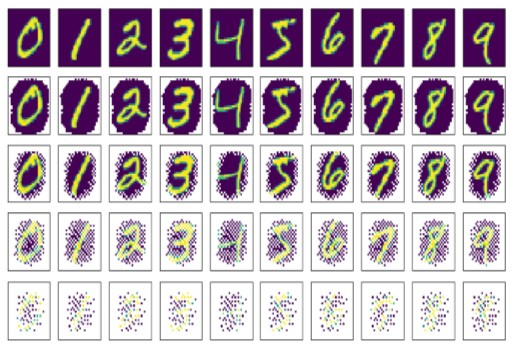
\includegraphics[scale = 1.0]{img/mnist reduced.jpg}
		\label{mi}
        \caption{Example of feature selection on MNIST dataset}
\end{figure}

\paragraph{Optimal Brain Surgeon algorithm (OBS).} This is another pruning algorithm, which focuses on the removal of a single connection, and it rescales all the weights in the network.

Consider a network which is trained to a local minimum in error $E$, i.e. the output of the back-propagation algorithm is $\min_{w \in \mathbb{R}^n} E(w)$. Then, we have that:

$$
\delta E = \bigleft( \frac{\partial E}{\partial w} \bigright)^T \cdot \delta w + \frac{1}{2} \delta w^T \cdot H \cdot \delta w + O(||\delta w||^3)
$$
, where:

\begin{itemize}
    \item $\delta E = E(w) - E(w + \delta w)$;
    \item $\bigleft( \frac{\partial E}{\partial w} \bigright)^T \cdot \delta w \approx 0$, because we're choosing the minimum $w$, so the partial derivative of $E$ is 0;
    \item $  O(||\delta w||^3) \approx 0$;
    \item $H = \frac{\partial^2 E}{\partial w^2}$ represents the Hessian matrix, containing all the second derivative information.
\end{itemize}

In this sense, removing a single connection means setting one of the weights, which will be called $w_q$, to 0, so as to minimize the increase in error $\delta E$. Thus, eliminating $w_q$ can be expressed as:

$$
\delta w_q + w_q = 0
$$

or 

$$
e_q^T \cdot \delta w + w_q = 0
$$
, where $e_q$ is the unit vector in the weight space corresponding to $w_q$, i.e. $e_q = [0 .. 1 .. 0]$, where the 1 is in position $q$. The final goal is then to solve the following constrained optimization problem:

$$
\min_q \min_{\delta w} \frac{1}{2} \delta w^T \cdot H \cdot \delta w \qquad \text{such that } e_q^T \cdot \delta w + w_q = 0
$$

We can transform this constrained problem into an unconstrained one using the \textbf{Lagrangian} (and by adding some more variables):

$$
L = \frac{1}{2} \delta w^T \cdot H \cdot \delta w + \lambda (e_q^T \cdot \delta w + w_q)
$$
, where $\lambda$ is the (undetermine) Lagrange multiplier. The goal now is to find the stationary points of $L$, i.e. points in which all its partial derivatives vanish. Tanking the partial derivatives and setting them to zero we obtain:

$$
\frac{\partial L}{\partial \delta w} = H \delta W + \lambda e_q = 0
$$

and

$$
\frac{\partial L}{\partial \lambda} = e_q^T \delta w + w_q = 0
$$

, from which we obtain that:

$$
\delta w = - \frac{w_q}{(H^{-1})_{qq}} H^{-1} \cdot e_q
$$

and 

$$
L = \frac{1}{2} \frac{w_q^2}{(H^{-1})_{qq}}
$$

, where $H^{-1}$ represents the inverse of the Hessian matrix, which is very computational demanding.

Finally, the algorithm proceeds as follows:

\begin{enumerate}
    \item Train a reasonably large network to minimum error;
    \item Compute $H^{-1}$;
    \item Find the $q$ that gives the smallest $L = \frac{1}{2} \frac{w_q^2}{(H^{-1})_{qq}}$. If this candidate error increase is much smaller than $E$, then the $q$-th weight should be deleted, and we proceed to step 4., otherwise, go to step 5.;
    \item Use the $q$ from step 3. to update all the weights $\delta w = - \frac{w_q}{(H^{-1})_{qq}} H^{-1} \cdot e_q$, and go to step 2.;
    \item No more weights can be deleted without large increases in $E$, so at this point we can re-train the network.
\end{enumerate}

There are some differences between the two pruning algorithms we considered:

\begin{itemize}
    \item In OBS we update all the weights;
    \item In OBS we assume that $O(||\delta w||^3) \approx 0$ and $\bigleft( \frac{\partial E}{\partial w} \bigright)^T \cdot \delta w \approx 0$;
    \item In OBS we assume that the network converges to the minimum;
    \item OBS algorithm is less efficient than Pelillo's.
\end{itemize}

